\begin{figure}[t]
\vskip 0.05in
\begin{center}
\centerline{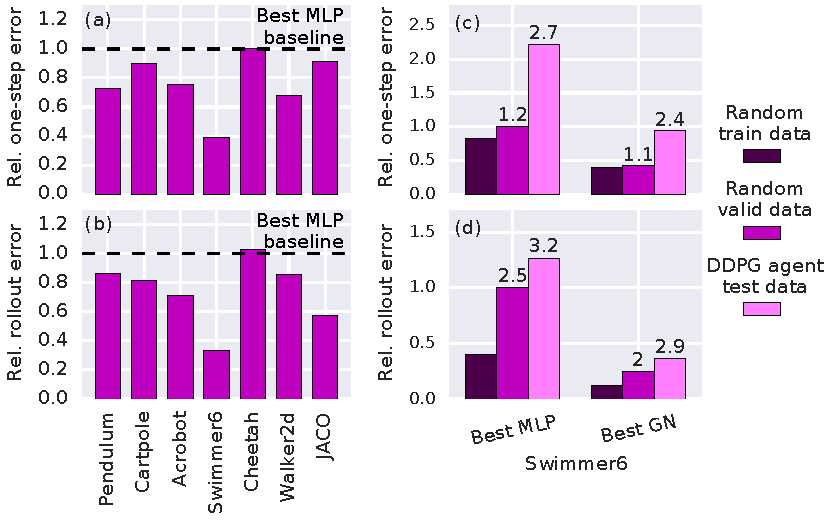
\includegraphics[width=\columnwidth]{figures/mlp_comparison_summary_swimmer6}}
\vspace{-0.1in}
\caption{Prediction errors, on (a) one-step and (b) 20-step evaluations, between the best MLP baseline and the best GN model after 72 hours of training.
Swimmer6 prediction errors, on (c) one-step and (d) 20-step evaluations, between the best MLP baseline and the best GN model for data in the training set (dark), data in the validation set (medium), and data from DDPG agent trajectories (light). The numbers above the bars indicate the ratio between the corresponding generalization test error (medium or light) and the training error (dark).
}
\label{fig:mlp_comparison}
\end{center}
\vskip -0.2in
\end{figure}